\documentclass[a4paper,10pt]{article}
\usepackage[margin=1.4in]{geometry}
\usepackage[swedish]{babel}
\usepackage[utf8]{inputenc}
\usepackage{titlesec}
\usepackage{titling}
\usepackage{todonotes}



\setlength{\parskip}{1em}
\setlength{\parindent}{0pt}
\titlespacing{\section}{0pt}{\parskip}{-\parskip}
\titlespacing{\subsection}{0pt}{\parskip}{-\parskip}
\titlespacing{\subsubsection}{0pt}{\parskip}{-\parskip}
\titlespacing{\part}{0pt}{\parskip}{-\parskip}

\externaldocument[kand-]{../Kandidatrapport/Kandidatrapport}
\externaldocument[krav-]{../Kravspec/kravspec}
\begin{document}
\def\ftitle{Kvalitetsplan}
\def\fversion{1.3}
\begin{titlepage} % Suppresses displaying the page number on the title page and the subsequent page counts as page 1
	\newcommand{\HRule}{\rule{\linewidth}{0.5mm}} % Defines a new command for horizontal lines, change thickness here

	\center % Centre everything on the page

	%------------------------------------------------
	%	Headings
	%------------------------------------------------

	\textsc{\LARGE Linköpings universitet \\ \vspace{0.2em} Institutionen för datavetenskap }\\[2cm]

    \large\today

    \vspace{1cm}


	%------------------------------------------------
	%	Title
	%------------------------------------------------

	\HRule\\[0.4cm]

	{\huge\bfseries Schemaläggningsstöd för  kirurgi \vspace{.1em} \\ \ftitle }\\[0.4cm] % Title of your document

	\HRule\\[1cm]

	%------------------------------------------------
	%	Author(s)
	%------------------------------------------------

	\begin{minipage}{0.7\textwidth}
			\large
            \emph{Version: \fversion}
            \vspace{1em}

            \textbf{\\Adam Andersson, Niclas Byrsten, \\Björn Hvass, Henrik Lindström, \\Martin Persson, Christoffer Sjöbergsson, \\Tor Utterborn}


            \vspace{1em}

            Handledare: Jonas Wallgren

            Examinator: Kristian Sandahl
	\end{minipage}
	~

	%------------------------------------------------
	%	Logo
	%------------------------------------------------

	%\vfill\vfill
	%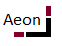
\includegraphics[width=0.2\textwidth]{../Templates/Aeon}\\[1cm] % Include a department/university logo - this will require the graphicx package

	%----------------------------------------------------------------------------------------

	\vfill % Push the date up 1/4 of the remaining page

\end{titlepage}


\section*{\begin{center}Projektidentitet\end{center}}
    \vspace{-2.5em}
    \begin{center}
        \begin{tabular}{|c c c|}
        \hline
        Namn & Roll & E-post \\
        \hline
        Adam Andersson& Teamleader & adam.e.a.andersson@gmail.com\\
        \hline
        Niclas Byrsten & Testansvarig & nicby889@student.liu.se\\
        \hline
        Björn Hvass & Konfigurationsansvarig & bjorn.hvass@gmail.com\\
        \hline
        Henrik Lindström & Utvecklingsledare & henli070@student.liu.se\\
        \hline
        Martin Persson & Arkitekturansvarig & marpe902@liu.student.se\\
        \hline
        Christoffer Sjöbersson & Analysansvarig & chrsj812@liu.student.se\\
        \hline
        Tor Utterborn & Dokument- \& Kvalitetsansvarig & tor.utterborn@gmail.com\\
        \hline
        \end{tabular}
    \end{center}

    \begin{center}
        \small
        \textbf{Kund}\\Region Östergötland, 581 91 Linköping.

        \textbf{Kontaktperson hos kund}\\
        Gunnar Nordqvist, IT-arkitekt, 010-1030698, Gunnar.Nordqvist@regionostergotland.se\\
        Erik Sundvall, Informationsarkitekt, 010-1036252, Erik.Sundvall@regionostergotland.se
    \end{center}

\vspace{9em}



\section*{\begin{center}Dokumentationshistorik\end{center}}
\begin{center}
 \begin{tabular}{|c c c c |}
 \hline
 Datum & händelse & iteration & version\\
 \hline
 2018-02-05 & Dokument skapas & 1 &  0.1\\
 \hline
  2018-02-16 & Konvertering till \textbf{\LaTeX} & 1 &  0.2\\
 \hline
   2018-02-19 & Version 1.0 färdigställd & 1 &  1.0\\
 \hline
   2018-03-04 & Revision av version 1.0  & 2 & 1.1\\
 \hline
    2018-04-23 & Tillägg sektion ``Kodstandard för TypeScript och JavaScript'' & 3 & 1.2\\
 \hline
     2018-05-16 & Tillägg sektion 4.1  & 4 & 1.3\\
 \hline
\end{tabular}
\clearpage
\end{center}
\tableofcontents
\clearpage
\section{Inledning}
\label{sec:Inledning}
Detta dokument beskriver kvalitetsarbetet i projekt att skapa ett schemaläggningsstöd för kirurgi till Region Östergötland.
\subsection{Syfte}
Syftet med denna kvalitetsplan är att beskriva de tekniker, aktiviteter och metoder som kommer att användas för att försäkra att en hög kvalitet hålls i projektet. Detta innebär att slutprodukten ska uppfylla alla krav, levereras i tid och hålla sig inom budgeten.
\subsection{Omfattning}
Detta dokument redogör för hur projektet skall uppnå sina högkvalitativa egenskaper och refererar till relevanta delar i projektdokumentation, se sektion \ref{sec:Refererade_dokument}.
\subsection{Refererade dokument}
\label{sec:Refererade_dokument}
Följande interna dokument refereras till i detta dokument:
\begin{itemize}
	\item Kandidatrapport
	\item Projektplan
	\item Kravspecifikation
	\item Testplan
\end{itemize}

\subsection{Definitioner, namn och förkortningar}
Följande lista definierar namn och termer som används i dokumentet.
\begin{itemize}
    \item JavaScript - Ett scriptspråk för webbutveckling
    \item Angular - Ett ramverk för gränssnitt till webbsidor
    \item WebStorm - En utvecklingsmiljö till JavaScript
    \item Git - Ett versionshanteringsverktyg
    \item GitLab - En webb-baserad versionshanterare som använder git
    \item Scrum - En agil utvecklingsmetodik
    \item Asana - Ett webb-baserat verktyg för projekthantering
    \item Typescript - Ett kodspråk med öppen källkod.
    \item TSLint - Ett statiskt kodanalys-verktyg som felsöker koden i realtid.
\end{itemize}

\section{Översiktlig kvalitetsplan}
Denna sektion ger en översikt av hur kvalitetsarbetet i projektet ska utföras.

\subsection{Organisation}

Projektgruppens kvalitetssamordnare är ansvarig för kvalitetssäkringen av projektet och  programvaran. Kvalitetsarbete ska utföras av samtliga projektmedlemmar men det är kvalitetssamordnaren som leder arbetet och har ansvar att utbilda och inspirera övriga medlemmar.

\subsection{Riskhantering}

För att kunna leverera en produkt som håller den kvalitet som utlovats så har risker för projektet identifierats och en riskbedömning av dessa tagits fram. \\
Se sektionen \emph{Riskhantering} i Projektplanen.

Riskbedömningen omfattar en värdering av sannolikheten av olika risker samt eventuell inverkan dessa skulle ha på projektet. En sammanslagning utav dessa två är en indikator på hur direkta hoten är mot kvaliteten i den levererade produkten.
En analytisk förstudie som omfattar dessa risker mot projektet i sin helhet och hur dessa skall undvikas går att läsa under sektionen \emph{Riskhantering} i Projektplanen.

\subsection{Verktyg}
\label{sec:Verktyg}

För att versionshantera kod så kommer GitLab att användas. På Google drive finns en mapp som delas med kund för att dela filer. WebStorm kommer användas som integrerad utvecklingsmiljö och Angular som webbramverk. Asana används som ett projekthanteringssystem.

Varje person ansvarar för att den är förtrogen med programvaror som används. Skulle det finnas osäkerhet så går det att fråga en annan projektmedlem. Vid behov så kan en medlem med kunskap hålla en genomgång för de andra.

\subsection{Standarder, rutiner och konventioner}
Denna sektion beskriver de standarder, rutiner och konventioner som ska följas under projektarbetet.

\subsubsection{Scrum}
\label{sec:Scrum}
För att få en så kvalitetssäkrande arbetsmetod som möjligt så valdes arbetsmetodiken Scrum. Nedan följer rutiner som kommer hållas för att säkerställa kvalitet.

\textbf{Dagliga Scrum-möten}\\
Varje dag gruppen möts hålls en snabb genomgång om vad som har åstadkommits sedan senaste mötet samt vad som skall presteras till nästkommande. Möjliga hot mot prestationer presenteras.

\textbf{Sprintplanering}\\
Projektet skall varannan vecka hålla en så kallad sprint planering. Planeringen går ut på att kravspecifikationen bryts ned i arbetsmoment som ska genomföras under nästa sprint. Arbetet följer de prioriteringar kund satt upp.

\textbf{Sprintgenomgång}\\
Efter varje sprint hålls en granskning av sprintens resultat där varje projektmedlem redovisar resultaten från föregående sprint.

\textbf{Sprintåterblick}\\
Det skall även hållas en s.k. sprintåterblick där gruppen analyserar kvaliteten på resultat samt diskuterar hur nästkommande sprint kan genomgå förbättringar.
Scrums iterativa arbetssätt ger projektet möjlighet att utvärdera och korrigera både produkten och processer utefter de önskemål som kunden framfört. Förhinder att uppnå den kvalitet som utsatts kan snabbt upptäckas och hanteras, se sektion \ref{sec:Kvalitetsmatning} om kvalitetsmätning.

\subsubsection{Pappersprototyper}
Vid tidig design av gränssnitt till produkten ska prototyper göras för att kunna få feedback från både gruppen och kunden. Prototyperna ska göras på papper eftersom detta är ett snabbt och effektivt sätt som inte kräver kunskap om något datorverktyg.

\subsubsection{Dokumentstandard}
För att alla dokument som skrivs i projektet ska ha ett konsekvent utseende och stil ska dokumentet Dokumentstandard skrivas och följas. Till denna ska det också finnas dokumentmallar som alla dokument ska bygga på.

\subsubsection{Kodstandard för TypeScript och JavaScript}
\label{sec:kodstandard}
I denna sektion beskrivs den kodstandard som ska följas vid kodning i TypeScript och JavaScript.
Gruppens kod exklusivt importerade bibliotek skall uppfylla de konfiguerbara regler som de statiska kodanalys-verktyget TSLint tillhandager.
Detta för att uppnå en hållbar standard inom läsbarhet, underhåll samt funktionallitet.

\textbf{Språk}
\begin{itemize}
\item All kod och alla kommentarer ska vara på engelska.
\end{itemize}

\textbf{Namngivning}
\begin{itemize}
\item Använd PascalCase för typer.
\item Använd camelCase för funktioner och variabler.
\item Använd CONSTANT\_CASE för konstanter och enumvärden.
\end{itemize}

\textbf{Stil}
\begin{itemize}
\item Öppnande måsvinge ska vara i slutet på raden (inte på ny rad).
\item Avsluta varje påstående med semikolon (även om det inte alltid krävs av språket).
\item Indentering görs med 2 blanksteg.
\end{itemize}

\subsection{Prestationer, resurser och planering}
För mjukvaruresurser se detta dokument, sektion \ref{sec:Verktyg}.
Den uppskattade tiden och andra resurser i projektet finns beskrivet under punkten Resurser i projektplanen.

\section{Aktiviteter, utfall och uppgifter}
Denna sektion behandlar aktiviteter, utfall och uppgifter för kvalitetssäkring av produkten och processen.
\subsection{Kvalitetssäkring av produkt}
Syftet med kvalitetssäkring av produkten är att skapa ett förtroende för kvaliteten på produkten. Detta innefattar all mjukvara samt alla dokument som skrivs under projektet. I denna sektion definieras de aktiviteter och uppgifter som krävs för att uppnå detta utfall.
\subsubsection{Utvärdering av planering}
För att på ett så entydigt sätt som möjligt klarlägga vad projektet har för standard så har en kravspecifikation utformats tillsammans med kund, se dokument Kravspecifikation.
Denna standard definierar projektets eftersträvade kvalitet enligt överensstämmelse med kund.
Kravspecifikationen är en grundpelare för den plan som utarbetats för projektet, som är beskriven i Projektplanen. Kraven representerar kundens behov, önskemål och förväntningar.
\subsubsection{Utvärdering av acceptanskrav för produkten}
Om berörda projektmedlemmar samtycker att delsystem är i ett sådant stadium att dessa kan testas för integration i systemet så skall testfall skrivas för delsystemen. När dessa delsystem godkänts i projektets testprotokoll enligt Testplanen, så integreras delsystemet i projektet.
\subsubsection{Utvärdering av underhåll för produkten}
I projektet inkluderas inte något underhåll av produkten eftersom det är en prototyp som kunden själv får vidareutveckla vid behov. Därför definieras inga aktiviteter eller uppgifter för detta.
\subsubsection{Hur produktens kvalitet ska mätas}
Produktens kvalitet ska mätas enligt de standarder och processer som beskrivs i detta dokument.
\subsection{Kvalitetssäkring av process}
Denna sektion beskriver de aktiviteter och uppgifter som krävs för att utvärdera att processerna som används i projektet räcker till och är effektiva.

\subsubsection{Utvärdering av processer}
För att den arbetsmetodik som följs i projektet ska hållas så effektiv som möjligt, ska den utvärderas och uppdateras på sprintåterblickarna i Scrum, se sektion \ref{sec:Scrum}.

\subsubsection{Utvärdering av miljöer}
De miljöer som används för utveckling samt dokument ska kontinuerligt utvärderas av alla projektets medlemmar. Eventuella synpunkter eller problem ska tas upp på nästa sprintåterblick i Scrum-arbetsmetodiken, se sektion \ref{sec:Scrum}.

\subsubsection{Mätning av processer}
En process kommer att mätas och detta är arbetsmetodiken som ska användas under projektet. Hur detta ska göras beskrivs i sektion \ref{sec:Kvalitetsmatning}, Kvalitetsmätning.

\subsubsection{Medlemmars kunskaper}
Se projektplan avsnitt \emph{Kunskap och färdigheter}.

\section{Ytterligare överväganden}
I denna sektion beskrivs ytterligare överväganden som måste behandlas under projektarbetet.
\subsection{Kvalitetsmätning}
\label{sec:Kvalitetsmatning}
Två kvalitetsmätningar skall hållas efter varje sprint för att värdera kvaliteten hos arbetsmetodik samt resulterande produkt.
Detta för att samtliga involverade i projektet på ett tidigt stadium skall känna till och förhålla sig till de föreskrivna kvalitetsmålen.

Ett användbarhetstest har även skapats för att mäta och fastslå grafiska komponenters användarvänlighet i produkten. Se avsnitt \ref{krav-subsec:kvalitetsakrav} i kravspecifikationen.

\subsection{Undantag och avvikelser}

Eftersom projektet skall utföras enligt en iterativ arbetsmetod så kommer den här planen samt de dokument den refererar till att revideras under projektets gång. Detta är nödvändigt för att uppnå den eftersträvade standarden. I den här planen presenteras en överblick av revisionerna i dokumenthistoriken.

\subsection{Iterativ arbetsmetodik}
När en arbetsuppgift bedömts att ej uppfylla de krav som specificerats i kravspecifikationen behöver uppgiften upprepas med en lämpligare arbetsmetod i en senare sprint. Se sektion \emph{Aktiviteter} i projektplanen samt sektion \ref{sec:Scrum} om Scrum i detta dokument.

\subsection{Risker med kvalitetssäkring av programvara}
Att följa denna kvalitetsplan medför de kända risker presenterade i avsnittet \emph{Riskhantering} i projektplanen. En risk är att kvalitetsplanen följs för febrilt, vilket kan medföra att frågan “Hur mycket får kvalitet kosta?” behöver ställas. Ansvaret att ställa denna fråga ligger på samtliga projektmedlemmar men främst på kvalitetssamordnare.

Den sistnämnda punkten förväntas hanteras av projektets iterativa arbetsmetodik Scrum som behandlas i sektion \ref{sec:Scrum}.

\subsection{Kommunikationsstrategi}
Internt skall arbetsgruppen föra en daglig kommunikation för att avstämma om arbetsflöde förhinder etc.
Externt (mot kund) skall avstämningar hållas veckovis för att fastställa krav och högkvalitativt arbete.

\end{document}
